\chapter{Mobile client}
\minitoc

\section{Lab Description}

\textit{The main objective of this assignment is to understand some of the some of the basic primitives and challenges of mobile computing.\\
You are required to expose Task manager’s Task entity as Google Endpoint (similar to the Todo item in the sample code) hosted on the Google App engine web application project, so that it can consumed by the mobile devises. Furthermore, also develop the functionality to send push notifications to the registered mobile devises whenever a new task is created on the app engine background. On the mobile application side, develop functionality for listing the tasks from the app engine background and also to display the push notification messages received from from the app engine backend whenever a new task is created on the app engine backend.}

\section{Solution}
The solution implemented makes use of the Android Development Tool Bundle; a collection of programs and tools assisting creation of software run on the Android platform. Using the Eclipe-integrated software suite the majority of the code needed to complete the assignment can be auto generated. During the development the Google plugin for Eclipse is also heavily used.\\
Communication between the parts of the distributed solution is handled by Google endpoints. These are classes that exposes methods for receiving and modifying data objects. Each endpoint is expected to expose a single data entity, as defined by the javax.persistence namespace. The endpoint framework manages the communication between endpoints by converting method calls to REST requests and method return type to REST responses (see \ref{rest_reflection}). Methods are identified by use of signature attributes defined in the com.google.api.server.spi.config namespace.\\
The solution consists of two eclipse projects: a backend and a client. The backend is deployed to the Google App Engine; a cloud service allowing for web services communicating via Google endpoints to be deployed and run on Googles dedicated servers. The client is an Android application communicating with the backend by use of Google endpoints.\\
In order to create the backend, a Task entity class is defined. This is a simple data object exposing the same data fields as the contents of task-manager-xml.xml. From this entity an endpoint exposing the entity can be generated. This endpoint provides functionality for receiving, adding, updating and deleting Tasks from the persistence managed by the service. Two additional endpoints are automatically set up to assists the program execution; one for transmitting device data, when a device registers for updates from the service, and one for sending and receiving message data. Persistence is managed by the framework, and accessed through the EntityManager class.\\
The Android clients control flow is entirely event driven. An application on this platform runs a number of activities, and these activities respond to events such as the screen being touched, or the device turning on and off. The application we create only run a single activity, RegisterActivity. This activity allows the user to register the device, so that it can receive notifications from the server. \\
We modify the TaskEndpoint class, so that insertion and updating of tasks triggers a broadcast message to all devices registered. The message contains a short list of the latest tasks to be added to the collection, printed out in a simple text format. We use a DeviceInfoEndpoint to gain access to the collection of devices that have registered to the service via RegisterActivity. We then simply iterate over this collection, and send the message to each device. In order to send the message we have to make use of the service´s API key; a unique number identifying the service on the Google App Engine. 


\section{Example Run}
In order to debug and run the client we are setting up a virtual Android machine that can execute the code.\\
A number of requests are send manually to the TaskEndpoint to create new Task objects on the server. Figure \ref{mobile_json_figure} shows the request to the server and the response. Consequently, a number of tasks are created on the site. Figure \ref{mobile_task_list_figure} shows a list of the tasks created.\\
\begin{figure}[ht]
	\centering
	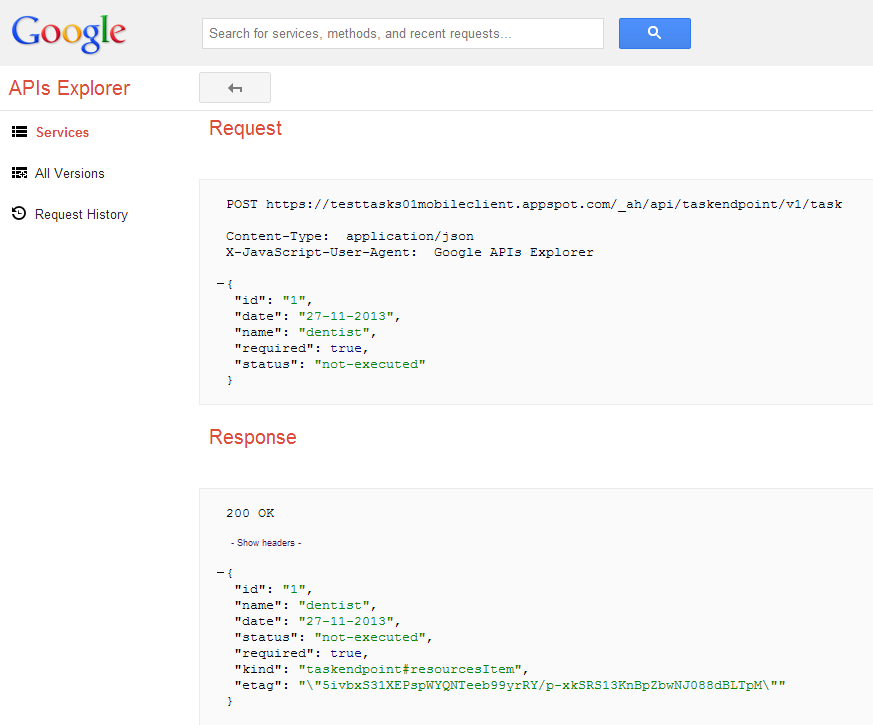
\includegraphics[scale=0.7]{images/googlecloud__createtask.png}
	\caption{creating a task}
	\label{mobile_json_figure}
\end{figure}
\begin{figure}[ht]
	\centering
	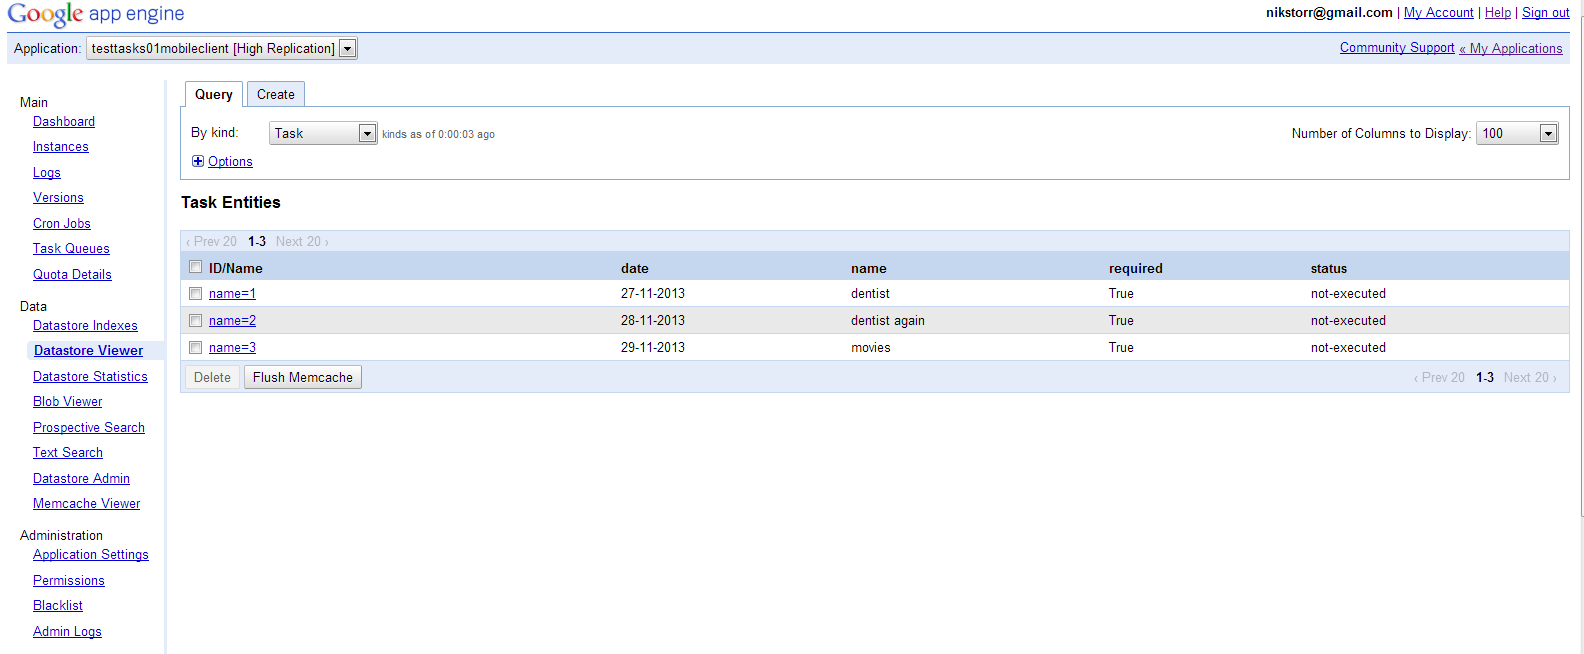
\includegraphics[scale=0.7]{images/googlecloud__taskexist.png}
	\caption{list of tasks created}
	\label{mobile_task_list_figure}
\end{figure}

The client is registered to receive updates whenever a new task is added to the Task collection. Figure \ref{mobile_registration_figure} shows the message informing that registration was successful.\\
\begin{figure}[ht]
	\centering
	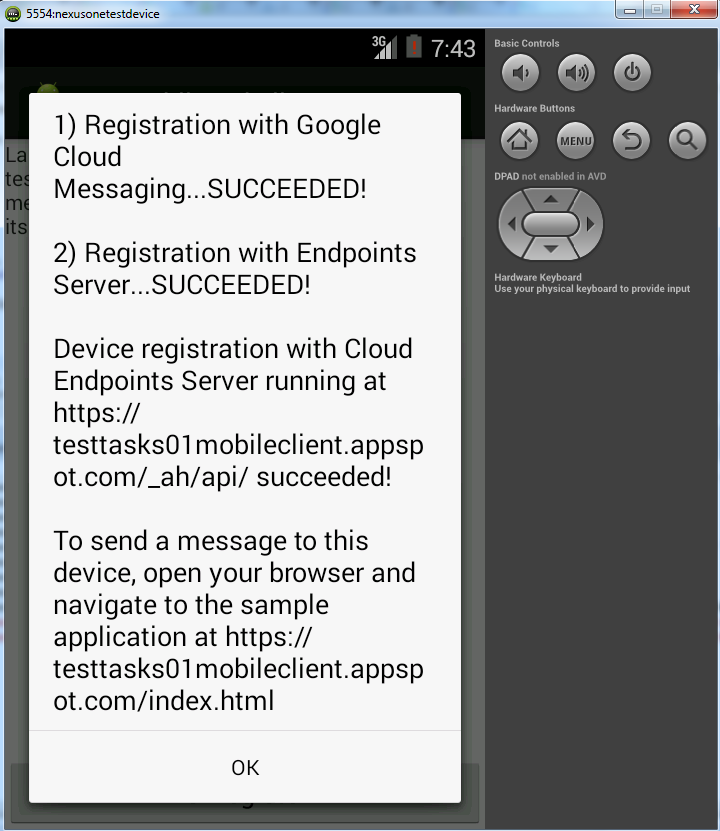
\includegraphics[scale=0.7]{images/googlemessagin_isonline_cloudmessaging.png}
	\caption{registration succeeds}
	\label{mobile_registration_figure}
\end{figure}

To test that communication happens properly a test message is sent manually. Figure \ref{mobile_message_figure} shows the message being sent at the server site, and figure \ref{mobile_hej_hej_hej_figure} shows the client receiving the message.\\
\begin{figure}[ht]
	\centering
	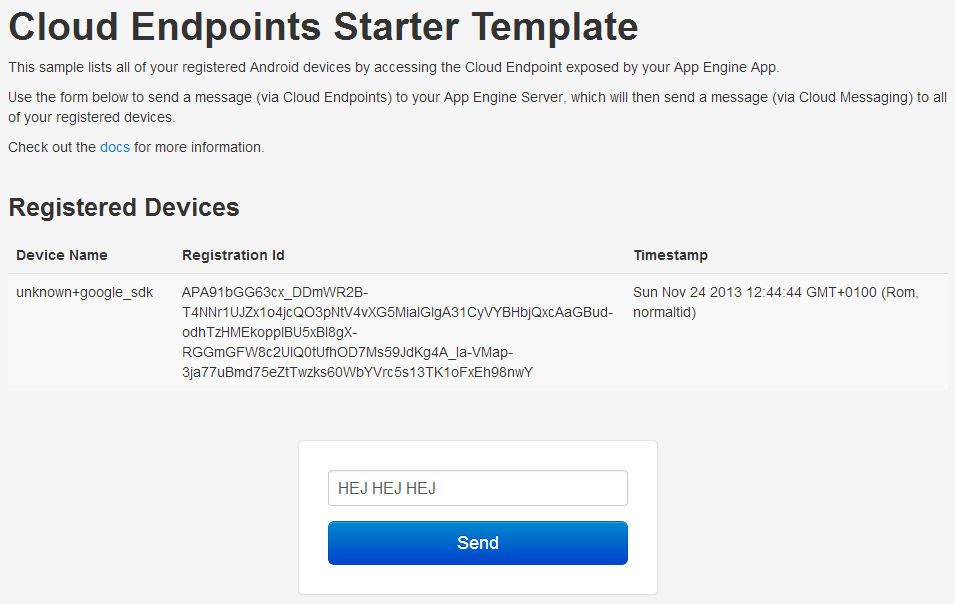
\includegraphics[scale=0.7]{images/googlemessagin_sendmessage.png}
	\caption{message being sent}
	\label{mobile_message_figure}
\end{figure}
\begin{figure}[ht]
	\centering
	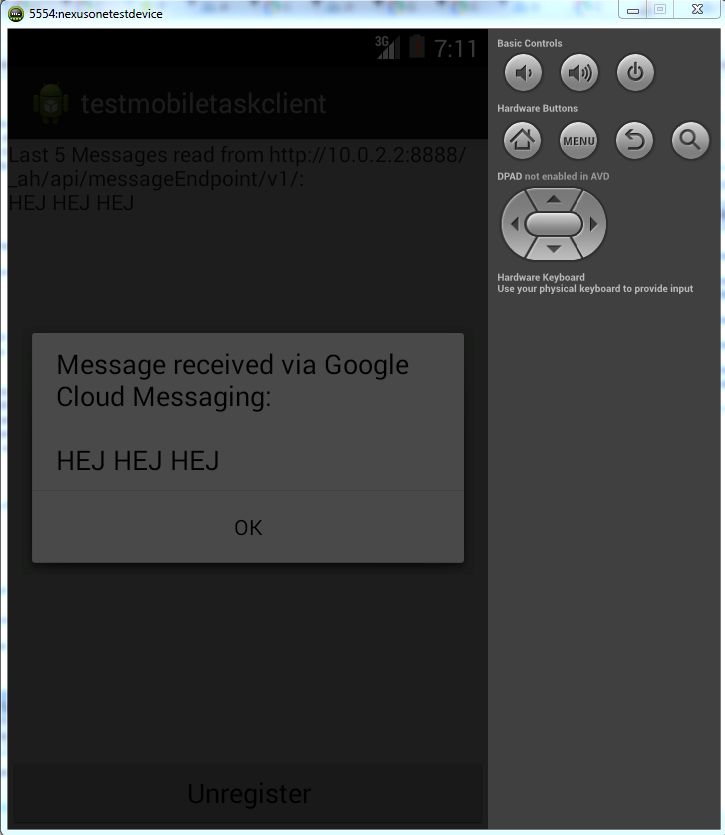
\includegraphics[scale=0.7]{images/googlecloudmessaging.png}
	\caption{message being received}
	\label{mobile_hej_hej_hej_figure}
\end{figure}

When a new Task is being created at the server site, the client receives the update message as shown in figure \ref{mobile_task_update_figure}.
\begin{figure}[ht]
	\centering
	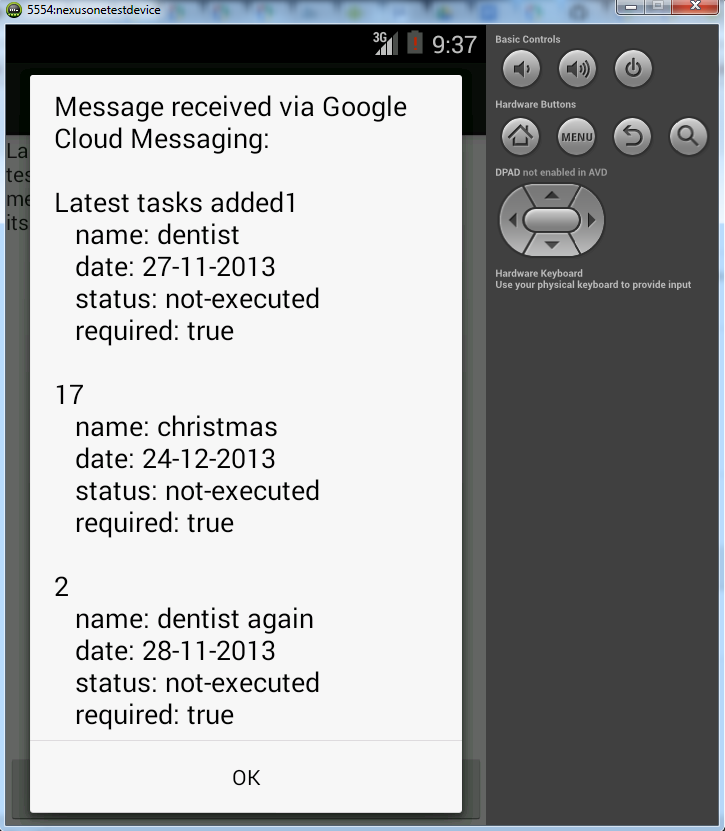
\includegraphics[scale=0.7]{images/googlecloud__tasksindevice.png}
	\caption{task update being received}
	\label{mobile_task_update_figure}
\end{figure}


\section{Theory}

Mobile computing (the connectedness of devices moving about in physical space ) and ubiquitous computing (the integration of computanional devices in physical space in everyday life) are, in this context, essentially the same in that they are both volatile i.e., change is the rule rather than the exception. As they move about physical space these computanional devices connect and disconnect to each other and the surrounding computational infrastructure. Mobile computing takes place \textit{between} physical spaces where ubiquitous computing is embedded into the physical space. \\

\begin{comment}
Because of this, mobile computing is considered 'volatile'.  \\ 
\end{comment}

\subsubsection{Volatility}
\label{volatility}
Volatility includes: failures of devices and communication links. Changes in bandwith (communication charateristics). Frequent creation and destruction of associations (between components). \\
 
Mobile and ubiquitous computing exhibits all of the above forms of volatility due to their integration into(and thus dynamic relation to) the physical world around them.\\


\subsubsection{Smart Spaces}
A smart space is any physical place with embedded devices in them. Mobile devices can enter and leave smart spaces in 4 ways.

\begin{itemize}
\item Physical movement: a \textit{device} may enter or leave a space. 
\item Logical mobility: a \textit{process} may enter or leave a space. 
\item Static devices may enter or leave the space e.g. a user may add or removeprocesses to her smart phone. 
\item Devices may fail i.e., dissapear from the space. 
\end{itemize}




However, the only matter of concern is whether a device/ process changes it's association with other processes i.e. a device either appear or dissappear from a smart space. Thus, it is irrelevant if a device /process is recident or visiting. Note some distinction is made as to the characteristics of connectivity in smart spaces e.g. the rate of association-change, or security issues (it matter which devices move in or out of a secure space). \\

\subsection{Device Model}
Ubiquitous and mobile computing leads to smaller and smaller devices which in turn puts restraints on energy supply and computing resources. This, taken into account in the following model.\\

\begin{itemize}
\item[Energy:] The smaller the device (assuming only battery powered devices ) the lower the battery capacity. This increases the propability of device failure and it poses a challenge to the frugality of algorithms applied.\\

\item[Resource constraints:] To make mobile and ubiquitous device physically small enough to embed in the physical space (e.g. to carry around), they naturally have less resources i.e processor speed, disc space and network bandwidth. How do we design algorithms that execute in a reasonable time and utilize resources in the surrounding space?\\

\item[Sensors and actuators:] To make devices context-aware (integrated in, and interaracting with the physical space) they are fitted with sensors and actuators e.g. a mobile phone may have a GPS fitted. In order to become ubiquitous these sensors are mass-produced, cheaply. Can we then trust them to function correctly/precisely ?  see P.839.\\

\item[Connectivity:] Devices have one or several wireless connectivities e.g. bluetooth, WiFi etc. The volatility of the connectivity has an impact on system properties e.g. Wireless disconnections are more likely than wired disconnections. A failure to process a request may be due to missing components somewhere else in the interconnected system. P. 841 \\ 


\item[Spontaneous interaction:] Components routinely connects and disconnects amongst themselves. we say that 
\textit{Associated} devices \textit{interact} i.e., devices can be associated without actually interacting. This poses a problem with security. What trust(privacy) can there be when devices spontaneously interacts and are spontaneously connected? E.g. if a sensor automatically registers users within its space and the users' other devices spontaneously interacts with other devices in this space this provides the opposite of security and privacy. The correlation between transactions on a creditcard and the movements of a user could reveal information. this is not a secure situation. \\
\end{itemize}

None the less, devices need to interoperate without the users' knowledge . This happens in two ways: 

\begin{itemize}
\item Network bootstrapping: A server within a smart space provides an IP address and DNS parameter which  devices queries. The server broadcast or multicast these informations. 
\item Association: When connected to a space, how do the device connect to the right process among possibly many ? and how do we constrain the communication to only devices within that particular space? \\

\textbf{The boundary principle} states that a space should define its boundaries as systems boundaries, not association boundaries (components from outside the space may connect to components within but the space may provide only the services belonging to it.) 
\end{itemize}

On way to solve the association problem is to use discovery services. 

\subsection{Discovery Services}

A discovery service is a directory service that takes into account volatile system properties [see section  \ref*{volatility}].  Device discovery and service discovery services exists. In device discovery the user selects among the available devices and queries that device for services offered. Service discovery happens automatically in situations where the user is concerned with the properties of the service, only.  \\

Discovery services has interfaces for \textit{registrering} (with a given address and attributes) and \textit{deregistering} services (note devices may dissappear without deregistering as per the properties of volatile systems!) and for \textit{lookup} of services. Each service matching a clients requests is returned with its address and attributes. Chosing a service is done by a secondary call (by the user, or automagically). \\

\subsubsection{Serverless Discovery}
Bootstrapping access to a local discovery service usually involves broadcasting(or multicasting) queries to a known IP address. Note this address must be know a priori by all devices. An alternative is to use \textit{serverless discovery} where devices collaborate to provide the directory service. There are two models. \textit{Push} and \textit{Pull}. In the push model services regularly multicast their descriptions. This comes at a price on bandwidth and energy use as devices continually push and listens for pushs. In the pull model clients multicast their queries and services respond (if their descriptions  match). In this model there's no wasted bandwidth but the client may receive several responses to a single request where one would do.\\

A device may leave without deregistering with a discovery service but the service needs to know as soon as possible, to maintain a fresh state. This can be achieved with \textit{leases}. A lease is an allocation of a resource with a build-in deadline., The client can renew the lease by repeating its request before the deadline (E.g. by calling a \textit{refresh()} method). Otherwise the service may reallocate the resource. Leases apply to services as well. Note there's a tradeoff between lease period and bandwitdh consumption.          \\

Remains; the issue of scope. How do we define the boundaries of a smart space? ways include having the user identifying himself to the service physically or by means of glyphs on a device. Other ways inlude physically constrained devices (devices whose reach are limited in space.) \\ 


\subsubsection{Real World Example:}
Android's 'discoveryListener' (a callback handler for registering services) involves handling a 'onServiceFound()', 'onServiceLost' and  'onServiceFailed()' methods.\\

The andriod NSD API then handles when services are found and lost etc.\\

Likewise the android system uses a ResolveListener callback to handle callbacks from the resolveService() method. The callback includes service information including an IP address and port number. 	\\

To preserve resources applications pause their discovery services when they become inactive and start them back up when they become active again. This is done with the onPause() and onResume() methods. Applications deregister with the DNS on exit by calling onDestroy() and tearDown() methods. 





\subsection{Interoperation}

Enough about connecting devices. Now we look at how devices interoperate.\\

The problem is heterogeneity. In a volatile environment the difference in component interfaces makes for a challenge. We seek to give devices a reasonable chance of interoperating with each other in, and between, spaces (the benefits of mobility can't be fully utilized if each space has its own programing  language). One approach is to allow heterogeneity, and to compensate for differences in interfaces by using adapters. This could potentially yield more than a lot of adapters. Another way is to try to constrain the syntax of the interfaces. Off course, using a single interface is much easier (and resource-friendly) than having to adapt to an ever increasing and varying number of different interfaces. This use of a simple unvarying interface is called a \textit{data-oriented} system. Data-oriented systems trade agreements on a set of functions for agreement on the types of data it accepts (the internet as a paramount example of a data-oriented system i.e., the HTTP protocol has limited interface... ).   \\

Note a system with a fixed interface still has to check compatibility between to components by means of either meta-data or by  verification of data sent to it. \\

\subsubsection{Interoperations Models}

Two ways of interoperation in volatile environments are events and tuple spaces. The subscription style communication in event based systems is clearly suitable for volatile systems but note that even here components can only operate correctly if they agree on the service and on the attributes and types of events i.e., they need agreements on the syntax and semantics used.\\ 


Aside, and to much amusement to the authors, XML does not provide a solution to the problem of interoperation in volatile systems, the problem of syntax and semantics. It merely provides a self-describing data structure. HahaHihi giggle giggle, hrmuphs (hate XML).\\

\subsubsection{Sensing And Context-wareness}

Apart from the volatility of mobile and ubiquitous computing, there is the matter of integration into the physical world, and context-aware systems. i.e., software fitted to sensors and how they respond to the sensed data. E.g. a cars brakes reacts differently when it is cold outside).\\ 

There are four challenges to context-aware systems. 

\begin{itemize}
\item Physical constraints (how to fit the sensor in the environment?). 
\item Abstraction from data (the same type of sensor may produce different data depending on the use.)  The application need som agreement from the sensors of the meaning of their data output. 
\item An application might need to combine sensor data to produce a reliable output (e.g. combine a camera  for face recognision with a microphone for voice detection.) 
\item Context changes (e.g. the device changes location spontaneously)
\end{itemize}



 




\section{Conclusion}